\documentclass{article}
\usepackage{tikz}

\begin{document}

A game of Tic-Tac-Toe played on a standard \(3 \times 3\) board. The winning hyperedges and the state of a proposed game are also given.

\begin{center}
    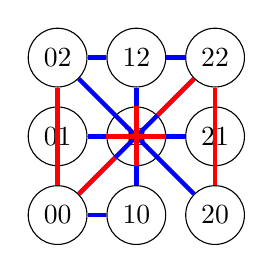
\begin{tikzpicture}[scale=1]
        % Draw the nodes
        \foreach \x in {0,1,2} {
            \foreach \y in {0,1,2} {
                \node[circle,draw,fill=white] (\x\y) at (\x,\y) {\x\y};
            }
        }

        % Draw the lines
        \draw[ultra thick, blue] (00) -- (22);
        \draw[ultra thick, blue] (02) -- (20);
        \draw[ultra thick, blue] (00) -- (02);
        \draw[ultra thick, blue] (20) -- (22);
        \draw[ultra thick, red] (01) -- (21);
        \draw[ultra thick, red] (10) -- (12);

        % Connect the winning hyperedges (lines)
        \draw[ultra thick, blue] (00) -- (10) -- (11) -- (12);
        \draw[ultra thick, blue] (21) -- (11) -- (01) -- (00);
        \draw[ultra thick, blue] (02) -- (12) -- (22);
        \draw[ultra thick, blue] (00) -- (01) -- (02);
        \draw[ultra thick, blue] (10) -- (11) -- (12);
        \draw[ultra thick, blue] (20) -- (21) -- (22);
        \draw[ultra thick, red] (00) -- (02);
        \draw[ultra thick, red] (20) -- (22);
        \draw[ultra thick, red] (00) -- (11) -- (22);

        % Add arrows if necessary
        % \draw[->, ultra thick, blue] (00) to (10);
        % \draw[->, ultra thick, blue] (10) to (11);
        % \draw[->, ultra thick, blue] (11) to (12);
        % \draw[->, ultra thick, blue] (02) to (12);
        % \draw[->, ultra thick, red] (01) to (11);
        % \draw[->, ultra thick, red] (11) to (21);
    \end{tikzpicture}
\end{center}

\end{document}